\documentclass{report}
\usepackage{graphicx}
\usepackage[ngerman]{babel}
\usepackage[utf8]{inputenc}
\usepackage[T1]{fontenc}
\usepackage{hyperref}
\usepackage{csquotes}
\usepackage[a4paper]{geometry}
\usepackage{underscore}
\usepackage[
    backend=biber,
    style=apa,
    sortlocale=de_DE,
    natbib=true,
    url=false,
    doi=false,
    sortcites=true,
    sorting=nyt,
    isbn=false,
    hyperref=true,
    backref=false,
    giveninits=false,
    eprint=false]{biblatex}
\addbibresource{../references/bibliography.bib}


\title{KI, Daten und Ethik}
\author{Nikolay Voropayev}
\date{\today}


\begin{document}

\maketitle

\abstract{
    In diesem Dokument wird grob erklaert wie KI funktioniert, es werden die Gefahren von KI analysiert, logisch behandelt und schlussfolgerungen gezogen, welchen beweisen sollen, dass: 
    \begin{enumerate}
        \item KI is nicht wirklich intelligent
        \item KI wird uns nicht ausloeschen wie in der Terminator Franchise.\citep{Terminator-Franchise}
        \item KI soll nicht nur in den haenden von Big-Tech Firmen ueberlassen werden, sondern sollte open-source gehalten werden.\citep{open-source}
        \item Datenschutz im zusammenhang mit KI is umsomehr wichtig als normalerweise.
    \end{enumerate}
}

\tableofcontents

\chapter{Einleitung}
\section{Was is KI?}
KI steht fuer "Kuenstilche Intelligenz", jedoch sieht KI gar nicht so aus wie ein menschliches Gehirn, welches aus Milliarden von Neuronen besteht.
KI's bestehen aus sogennanten Neuronalen Netzwerken. \citep{neural-networks}
\begin{figure}[h]
    \centering 
    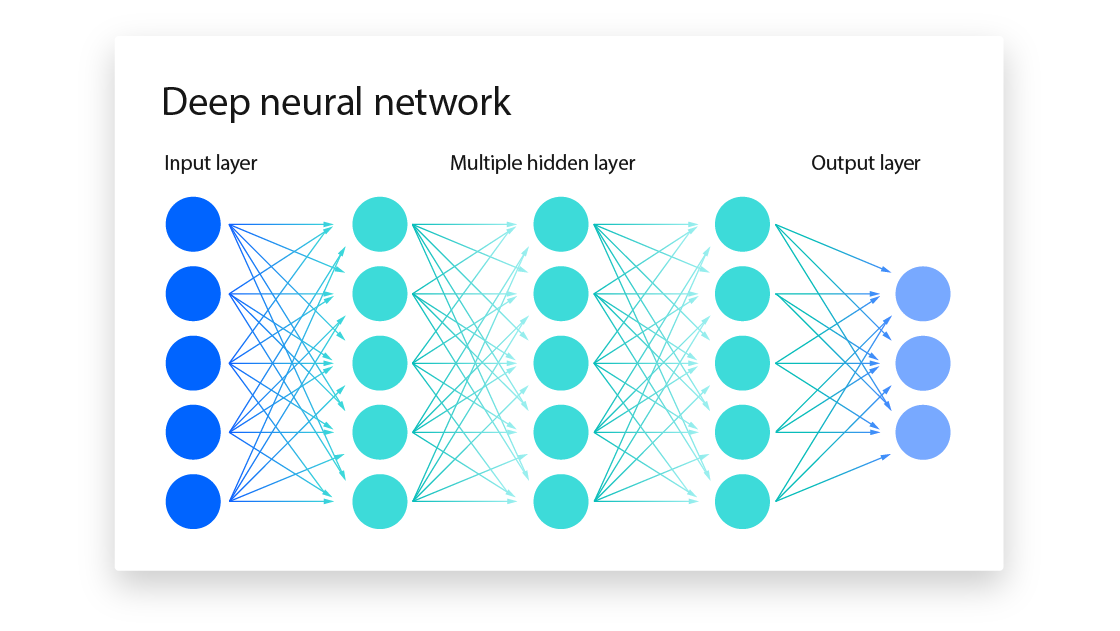
\includegraphics[width=1\textwidth]{NN-ibm.png} 
    \caption{Neurale-Netzwerk-Grafik, IBM}
    \label{fig:meme}
\end{figure}
\newline
Ich werde in dieser Arbeit nicht in die Mathematischen details eingehen, auch nicht den Unterschied zwischen KI und "Machine Learning" \Citep{machine-learning-ibm} erklaeren, da dies fuer diese Arbeit nicht besdonders wichtig ist. Einfach erklaert beruht Machine Learning mehr auf menschlichen Eingriffen, wahernd "tiefes" Lernen auf vielen "Schichten" der KI beruht. Was mit Schichten gemint ist, wird weiter unten erklaert. Auch wie diese Neuronalen Netzwerke funktionieren wird auf der IBM-website \citep{ai-ibm} gut erklaert. Ich bin kein KI-Ingineur und kann dewswegen nur die Erklaerungen von anderen Zitieren oder mein oberflaechliches Verstandnis davon in Worte fassen.
\subsection{Was sind Neuranale Netzwerke?}
Einfach erklaert, haben Neurale Netzwerke wie in der Abbildung Schichten. in jeder dieser Schichten gibt es Schnittpunkte. Wenn ein bestimmter Input einen Schnittpunkt aktiviert, sendet dieser einen bestimmten Output weiter. Wie stark dieser Output gewichtet ist, und wie er verarbeitet wird, haengt von dem Netzwerk ab.
Das wichtigste ist aber, dass man nicht wissen kann, was in diesen Netzwerken passiert, und warum ein bestimmter Input so wahrgenommen wird, wie er wird. Dies ist fuer spaeter wichtig.
\newline
Falls es schwer faellt, dies im Textformat zu verstehen, kann dieses Video \citep{how-ai-is-trained} dabei helfen. Der betreiber dieses Youtube-Kanals hat auch selber seine eigene KI trainiert.

\section{Was ist Datenschutz und warum ist es wichtig?}
Per mirriam-webster \citep{data-def} sind Daten faktuelle Informationen.
Jedoch wenn wir von Daten im bezug auf Datenschutz sprechen, sind nicht einfach Statistiken zum Schokoladen-Konsum des Durchschnittlichen Schweizers, welches ueber 10kg pro kopf pro jahr betraegt \citep{schokoladenkonsum-pro-kops-schweiz},
sondern es geht um Informationen, wie Lokationsdaten, die durch Bluetooth, WLAN oder Mobilfunknetze durch triangulation ausgerechnet werden koennen. Oder Kaufgewohnheiten durch die Ausgabensdaten der Kredikarten.
Viele solche Daten koennen aus anderen "herausgelesen" werden. Manche schlussfolgerungen zu schliessen ist es jedoch nicht moeglich fuer ein klassisches Computer-Programm.
\newline
\newline
Datenschutz ist der Prozess der minimierung von der Menge dieser Daten, welche aufgezeichnet werden. Zum beispiel durch das verwenden von verschluesselung kann der Inhalt einer Nachricht unzugaenglich gemacht werden. Dabei sind aber die Meta-Daten \citep{metadata} nicht unbedingt unsichtbar. Wenn die IP-Adresse, von der eine Nachricht gesendt worden ist und die Uhrzeit zugaenglich ist, kann genau bestimmt werden, wer diese Nachricht gesendt hat. Dies ist ein sehr grobes beispiel und Meta-Daten werden von Gerichten benutzt um zu entscheiden, ob Jemand Verhaftet werden sollte oder nicht. 
\newline
\newline
Das am weitesten verbreitete benutzen von Mata-Daten ist das sogennante Geofencing.\citep{geofencing}
\subsection{Warum ist Datenschutz wichtig?}
Dies ist ein sehr komplexes Thema und es gibt endlos Informationen dazu. Da es aber immer gut ist eine eigene Meinung zu bilden, werde ich einfach nur Beispiele bringen, warum Datenschutz wichtig sein kann. Es gibt viele Personen, welche sagen "Ich habe nichts zu verstecken." Darauf gibt es ein gutes Beispiel, um zu visualisieren, warum das nicht so stimmt. Falls das so ist, waere diese Person damit Einverstanden, mir zugang zu allen ihren Konversationen, allen Photos, allen Daten auf ihren Geraten zu geben? Wahrschleinlich nicht, und das ist gut so. Auch wenn eine Firma die Daten nicht weiterverkauft, Hacker bekommen zugriff die ganze Zeit zu diesen Datenbanken, und diese betriben dann Identitaetsdiebstahl. 
\newline
Es gibt zalreiche vorfaelle bei denen zum Beispiel Versicherungs-Premien von Autofahrern in den Vereinigten Staaten hoeher wurde, weil sie stark gebremst haben, und wahrschleinlich ein KI entschieden hatte, dass dieser Autofaherer schlecht auto faheren kann. Auch wenn er in einer Situation bremste, in der er einen Unfall verhinderte. CNN hat dieses Problem publiziert. \citep{car-syping-cnn}
\newline
Aber dies ist nur eine Art, auf die unregulierter oder inkompetenter umgang mit Daten verherende Folgen hat, es gibt, wie ich schon erwaehnt habe, endlos solche beispiele.
\newline
Es gibt sehr viel Videos auf Youtube darueber, welche viel besse als ich es erklaeren koennte, zu diesem Thema erklaerungen bereitstellen, und dieser Youtube-Kanal \citep{tha-hated-one-yt-channel} laesst fuer alle Informationen Quellen, dadurch ist es einfach die Informationen zu verarbeiten und sie koennen ueberprueft werden.
Ich wuerde empfehlen die unten gelisteten Videos anzuschauen.

Apple and Google contact tracing is a dystopian nightmare \citep{contact-tracing}

Google vs DuckDuckGo Search engine manipulation, censorship and why you should switch \citep{google-DuckDuckGo}

Google will spy on you in physical stores Can businesses really do anything? \citep{offline-tracking-google}

Your Car Is a Better Spy than Facebook \citep{car-better-spy-than-facebook}

Don't use WhatsApp!\citep{dont-use-whatsapp}

Your Keystrokes Are In The Cloud \citep{you-keystrokes-are-in-the-cloud}
\newline
Falls man die Zeit hat, wuerde ich auch empfehlen, 1984 von George Orwell und 451 Fahrenheit von Ray Bredberry zu lesen, es sind sehr Spannende Buecher und sie haben mit der Thematik vieles gemeinsam.
Netuerlich ist dies alles nicht noetig, einfach um zu verstehen, warum Datenschutz wichtig ist, Die wichtigsten Quellen werden speater angegeben und werden auch markiert sein, das sie fuer ein verstaendnis noetig sind. Aber das wissen vom monumentalem Aussmass dieser Probleme ist nuetzlich. 
\chapter{KI, Daten und Ethik}
\section{KI und Daten}
Wie schon frueher erwaehnt, stellt KI neue moeglichkeiten for, Informationen zu verarbeiten. Ungluegcklicherweise bedeutet dies, dass eine KI Daten viel besser verarbeiten kann.
Die Social-Media-Platform \hyperlink{reddit.com}{Reddit} zum Beispiel verkauft alle Benutzer-Generierte Daten an OpenAI, eine KI-firma, welche hauptsaechlich Microsoft gehoert. \citep{openai-site}
Hier von der offieziellen Website von OpenAI. \citep{openai-reddit-deal}
\newline
\newline
Technologien entwicklen sich sehr schnell, viel schneller als entsprechende Gesetze eingefuehrt werden koennen. So wurden zum Beispiel Deep-Fakes \citep{deepfakes}, welche massive schaeden verursacht haben \citep{deepfakes-scam}, erst vor kurzen von Politikern als Problem anerkannt.
\newline
\newline
Das schockierendste ist, das es schon jetzt Socia-Credit-Scores gibt, die nicht von einem Diktaturstaat, sondern von Geschaeften, Banken und Versicherungsfirmen benutzt werden, um Kunden auf ihre "Wertigkeit" zu gradieren. All dies moeglich durch KI.
Das Problem damit, KI zu erlauben dies zu tun ist das KI mit denen Daten arbeitet, die es bekommt. Dies ist spaeter wichtig.
\citep{ai-social-credit-scores} Dieses Video ist fuer das Verstaendnis notwendig
\newline
\newline
Es gibt auch eine grosse Luege, welche alle Big-Tech KI-Firmen immer wieder erzaehlen. Naehmlich sollte KI gefaehrlich sein, und es sollten nur bestimmte Firmen die erlaubnis haben, KI zu erstellen. Dies sollte durch Gesetze geregelt werden, die es schwer machen, ein eigenes, open-source KI-Modell selber herzustellen, und ja, dies ist moeglich, und sogar realativ einfach, denn es gibt videos, in denen Youtuber eine einfache KI trainieren, um zum beispiel das bestmoegliche keyboard-layout fuer bestimmte kriterien. Deswegen wollen Big-Tech Firmen den Zugang ueber Lizensen sperren. \citep{training-an-ai-model}
\newline
Es gibt sogar ein Dokument, welches von einem Google-Mitarbeiter geschrieben worde, in welchem beschreiben wird, wie open source modelle besser sind, als die, welche von Big-Tech erstellt werden und wie es unmoeglich ist, dagegen fair zu gewinnen. \citep{google-enginner-says-big-ai-sucks}
\newline
\citep{ai-extinction-lie} Dieses Video ist fuer das Verstaendnis notwendig. Es beschreibt die Luege von Big-Tech sehr genau und erklaert auch warum es eine Luege ist und nicht die Wahrheit.
\newline
\newline
Aber es wird noch schlimmer, KI verbraucht unemngen an Wasser, so viel wasser, dass Big-Tech-AI "Kriege" um wasserreserven ausloest. Richter muessen entscheiden, ob sie mehr Wasser and Bauern, Einwohner von Staedten, oder an die Datenzentren, welche die KI's prozessieren, einteilen.
In den USA gibt es deswegen ein Wasserprbolem in manchen Regionen. \citep{ai-water-wars}
\newline
\newline
Es gab einen ziemlich bekannten Vorfall, bei dem ein US-Resident fotos seines Sohnes waehrend der Covid-19 Pandemie fuer den Artzt nahm. Der Mann benutzte Google Photos. Das KI welches illegale materialien erkennen sollte, entschied die Fotos seien Pornografische bilder eines Kindes, und nach einer weile klopfte die Polizei an seiner Tuere. \citep{google-photos-false-flagging}

\section{Skynet im echten leben}
Wie ich schon vorher erwaehnt habe, ist KI nicht wirklich Intelligent, aber durch die oben genannten anwendungszwecke kann KI sehr guet sogar Kriege ausloesen. Und zwar echte Kriege.
\newline
Sagen wir mal es gibt ein Land, welches Konkurrenz zur derzeitigen Weltmacht leistet. Die Klassischen wege die Konkurrenz zu schwaechen funktionieren nicht, das Land entwickelt sich weiter und Propaganda kann ihm nichgts antun. In ihrer verzweifulng die Spitze zu behalten nimmt die Weltmacht drastische Massnahmen: Sie erlauben KI im Militar zu benutzen, autonome Waffen werden eingesetzt. Es funktioniert perfekt, die Konkurrenten mit ihren fleischigen Soldaten koennen mit der geschwindigkeit, mit der Computer arbeiten nicht mithalten. Einige Jahre spaeter stellt sich jedoch heraus, dass die KI nicht nur Soldaten angegriffen hatte, sonder in den Tausenden zivilisten umbrachte. Dies war zu erwarten, denn wie im ersten Kapitel erwaehnt, wenn KI fehler macht, kann man diese nicht wirklich beheben. Man kann nur das ganze Model weider neu aufbauen. Deswegen sind kleinere Modelle beliebter, vor allem in der Open-source-Welt.
\newline
\newline
Die geschilderte Situation Toent sehr Dystopisch und man wuerde denken, das koennte nie im echten leben Passieren, nur, es ischt schon Passiert. Die gruende fuer welche die USA ihren Drohnenkrieg startete war zwar nicht so einfach und die diskussion von ethik von krieg und terrorismus ist nicht zewck dieser Arbeit, aber die Tatsache, dass unzaehlige Zivilisten von Machinien umgebracht wurden, weil ein KI so entschied, bleibt stehen.
Den Drohnenkrieg zu beschreiben ueberlasse ich professionellen journalisten der SRF. \citep{drones-srf}
\newline
Wie schon vorher erwaehnt, es gibt "Social-credit-scores" welche von betrieben personen gegeben werden. Banken sind ein gutes Beispiel dafuer. Das grosse Problem damit ist, dass diese KI's oft wenig Objektiv ist, denn die Daten, aus denen ein theoretisch objektiver Algorythmus wird zum Beispiel rassistisch, oder das Bekannte Amazon-AI, welches benutzt wurde um Arbeits-Kandidaten zu evaluieren. Diese KI "lernte" nach einer Weile, dass Frauen schlechte Arbeiter sind, und nach mehreren versuchen den Algorythmus zu korrigieren, wurde das ganze Programm eingestellt und "Subjektive" Menschen wurden wieder verwendet.
\newline 
Ein sehr beliebtes Beispiel ist der Youtube-Algorythmus. Nach nur ein paar Minuten nachschlagen kann man buchstaeblich hunderte oder gar tausende Faelle finden, in denen die KI komplett grundlos ein Video geloescht wurde, oder jemand der die Rechte zu Copytight-Geschuetztes Material eine Warnung bekam, dass es verboten sei, Copyright-Material zu verbreiten, obwohl diese Person die Rechte hat.
\newline
Kurzgefasst, es ist eine schlechte Idee, KI ueber Probleme von Menschen entscheiden zu lassen. Das Buch "Watchbirds" ist eine gute Illustration davon. Falls dies immer noch nicht genug Informationen sind, um zu beweisen, dass KI problematisch ist, dann sollte dieses
Dokument \citep{google-enginner-says-big-ai-sucks}
eines google-KI-Ingenineurs es beweisen.
\section{Arbeitsplaetze und KI}
Es ist ein weit verbreiteter Konsensus, das KI Arbeitsplaetze stehlen wuerde und dadurch unethisch ist. Das stimmt nicht, es gibt zwar Arbeitsgeber welche glauben, sie koennten ihre Arbeiter durch KI ersetzen, aber die meisten dieser Arbeitsplaetze koennen auch ohne KI automatisiert werden, werden aber nicht. Auch darf man nicht vergessen, das KI sich nicht unendlich verbessert, und je mehr KI-generierte Materialien im Internet verfuegbar sind, desto langsamer wird die Entwicklung der KI, da diese Daten die KI "vergiften". Dies passiert, weil ein KI ja menschengemachte Texte imitieren sollte, jedoch wenn diese KI auf vielen KI-generierten Texten trainiert wird, wird es andere KI-generierete Texte imitieren. Also aehnlich wie die kombinierung von verwandter DNA zu fehlbildungen fuehrt, genause sollte KI nur auf guten Daten trainiert werden. 
\newline
\newline

\printbibliography
\end{document}
